\chapter{Implementation} \label{Implementation}

\section{Front End}

\subsection{The SCIONLab Website}

In the configuration form for user-\acsp{AS} of \acs{SCIONLab}'s web interface, I added the \ac{HTML} code snippet visible in listing \ref{HTML code}. This results in an additional text input field (as visible in figure \ref{User-AS Configuration Form}) that allows the user to add an upper limit for the bandwidth. If the user then clicks the \textbf{Create \acs{AS}} button, the input from that field is read into the data model. Updating the configuration of an existing \acs{AS} works similarly.

\begin{lstlisting}[language=html, caption = HTML code snippet of the bandwidth field from user\_as\_form.html, captionpos=b, numbers=left, frame=single, breaklines=true, breakatwhitespace=true, showstringspaces=false, label=HTML code]
<div class="form-group has-feedback">
  {{ form.bw_limit.label }}
  <div class="input-group">
    
    <div class="input-group-append">
      <span class="input-group-text bg-white">
        <span class="fa fa-tachometer"/>
      </span>
    </div>
  </div>
</div>
\end{lstlisting}

\begin{figure}[H]
	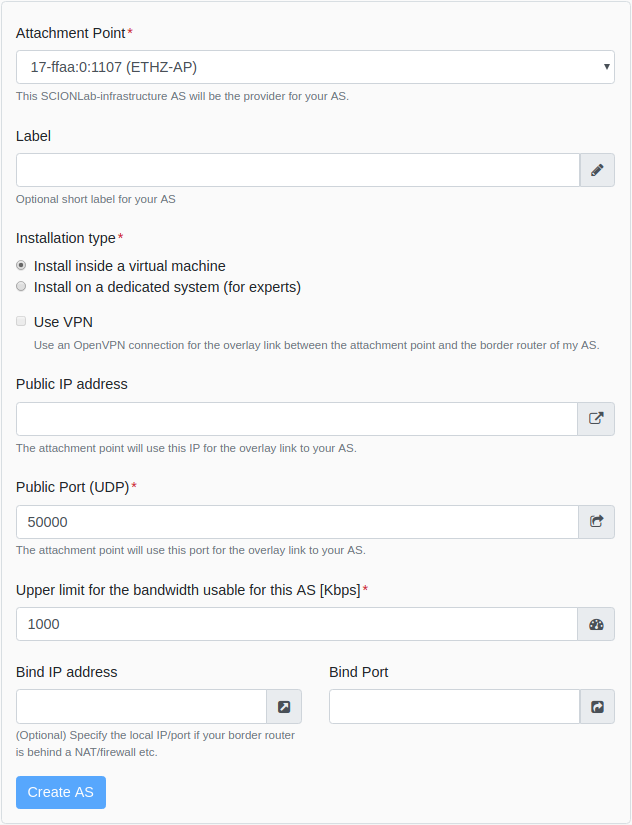
\includegraphics[width=0.7\textwidth]{img/user_as_form.png}
	\centering
	\caption{User-AS Configuration Form}
	\label{User-AS Configuration Form}
\end{figure}

\subsection{The Data Model}

The \acs{SCIONLab} server is based on the Django framework. Therefore \acs{SCIONLab}'s data model is based on Django's data model as showed in figure \ref{Django Model Dependency Diagram}. The bandwidth limit is stored as an attribute in the \textit{Link} class. As visible in figure \ref{Django Model Dependency Diagram}, the \textit{Host} class can access all of its interfaces and therefore also all of its links. The \textit{Host} class represents the \acs{VM}, container or physical machine hosting the \acs{SCION} services. Since the host can access all information we need to generate the \textit{link\_info.json} file, we hand a host object as an argument into the function \textit{generate\_link\_info(host)} of the file \textit{bandwidth\_config.py}. This function returns a dictionary which is used in the \textit{config\_tar.py} file to generate a \acs{JSON} file and add the \textit{link\_info.json} file to the tarball that is later deployed to the \acl{AP}.

\begin{figure}[H]
	\centering
	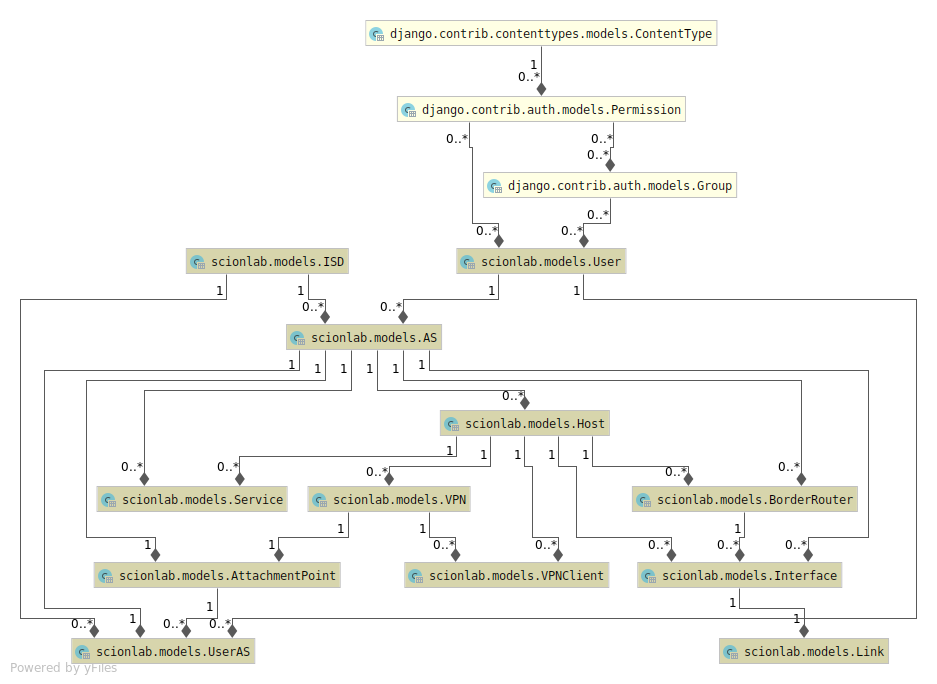
\includegraphics[width=0.8\textwidth]{img/Django_diagram.png}
	\caption{Django Model Dependency Diagram}
	\label{Django Model Dependency Diagram}
\end{figure}

\subsection{Attachment Point Configuration}
On the \aclp{AP} there will be a python file called \textit{scionlab\_config.py}. This file is responsible for configuring the \acsp{AP} and to start the \acs{SCION} services. Since the \acs{SCION} services get restarted after each reboot and whenever the configuration changed, it is sufficient to invoke the \textit{scionlab\_bw\_limiter} and enforce the limitations at this point.
%TODO check if this is accurate 
It is important to note that \acs{TC} configurations get automatically reset after each reboot and therefore need to be re-enforced every time the \acs{AP} restarts.

\section{Back End}

The back end consists mainly of the python files listed below. Additionally there are some \acs{JSON}-files that are used to either safe some settings or store some text that would take up too much space in the code and is therefore put into a separate file for the sake of readability. The python files have the following functionality:

\begin{enumerate}
\item[$\bullet$]\textit{scionlab\_bw\_limiter}:
\\
This file implements the entry point of the entire program. It parses command line arguments, let's you configure the default bandwidth and the path to the \textit{link\_info.json} file and invokes the \textit{bandwidth\_configurator.py} in order to enforce or reset bandwidth limitations or to show the current \acs{TC} configuration. It accepts the following options:
	\begin{enumerate}
	\item[\textit{-h}:] Show help text that explains how to use the program. This text is stored in the \textit{config\_files/help.json} file.
	\item[\textit{-l}:] Enforce the bandwidth limitations according to the \textit{link\_info.json} file.
	\item[\textit{-r}:] Reset any previously set \acs{TC} configurations.
	\item[\textit{-s}:] Show the current \acs{TC} configuration.
	\item[\textit{-b}:] Set or update the default bandwidth. This takes as an argument a positive integer, which represents the default bandwidth in kilo bits per second.
	\item[\textit{-p}:] Set or update the path to the \textit{link\_info.json} file. This option takes the path to that file as an argument.
	\end{enumerate}

\item[$\bullet$]\textit{code\_base/bandwidth\_configurator.py}:
\\
This file contains the implementation of the \textit{limit()}, \textit{reset()} and \textit{show()} functions. The \textit{limit()} function reads in the \textit{link\_info.json} file and creates link objects accordingly. Then it sets up the virtual interfaces, creates the \acs{TC} logic and invokes the \textit{make()} function from the \textit{tc\_logic.py} file. The \textit{reset()} function simply deletes the root \acs{QDISC} as well as the ingress \acs{QDISC} for each used interface. And finally the \textit{show()} function is responsible for printing out the current \acs{TC} configuration.

\item[$\bullet$]\textit{code\_base/cmd\_executor.py}:
\\
The command executor implements some static helper functions, that simplify running a command on the command line. One function silently runs a command using the subprocess \acs{API}, an other one runs a command and prints it to the console, one runs the command silently but returns the output it received by running the command and finally one function runs a command after it printed it and returns the output.

\item[$\bullet$]\textit{code\_base/constants.py}:
\\
This file contains some static variables that are constant throughout the entire program. 

\item[$\bullet$]\textit{code\_base/interfaces.py}:
\\
This file is used to retrieve information about the interfaces configured on the host machine and bundle it together in interface objects.

\item[$\bullet$]\textit{code\_base/links.py}:
\\
Analogously to the \textit{interfaces.py} file the \textit{links.py} file is used to bundle together information about links. This information is parsed form the \textit{link\_info.json} file. Furthermore, in this file the virtual interfaces are set up and mapped to their corresponding physical counterpart.

\item[$\bullet$]\textit{code\_base/systeminfo.py}:
\\
The \textit{systeminfo.py} file is used to retrieve some information about the host like whether a file exists or which interface is used by default.

\item[$\bullet$]\textit{code\_base/tc\_command\_generator.py}:
\\
The \acs{TC} command generator is used to generate the \acs{TC} commands that are used in order to configure the system. The generation functions return these commands as strings. They are later executed using the command executor.

\item[$\bullet$]\textit{code\_base/tc\_logic.py}:
\\
This file is the centrepiece of the entire program. It defines the building blocks to build up the entire logic of our \acs{TC} hierarchy according to figure \ref{QDISC-Set-up}. The \ac{UML}-model in figure \ref{tc logic uml} visualizes the relevant building blocks and their attributes and functions. The most interesting function is probably the \textit{make()} function. It first uses the \acs{TC} command generator to get the command to turn it's properties into \acs{TC} configurations, executes the command using the command executor and then recursively calls \textit{make()} on the building blocks that are lower down in the hierarchy tree. Like this the entire \acs{TC} logic can be turned into \acs{TC} configuration on the host. 

\item[$\bullet$]\textit{code\_base/virtual\_interfaces\_manager.py}:
\\
The virtual interface manager is used to set up and delete the virtual interface and to map them to their physical counterparts.

\end{enumerate}

\begin{figure}[h]
	\centering
  	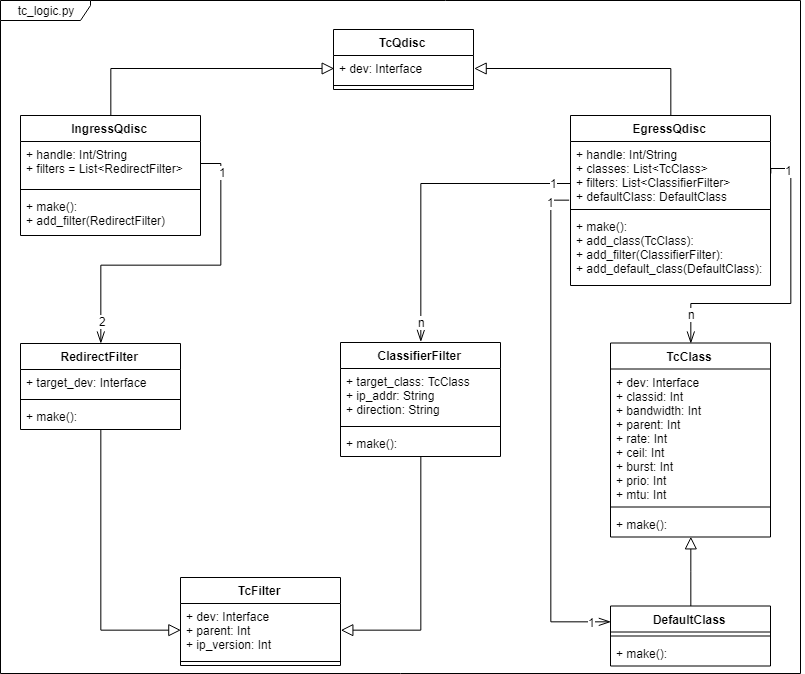
\includegraphics[width=\textwidth]{img/tc_logic_uml.png}
    \caption{UML-Model of \text{tc\_logic.py}}
    \label{tc logic uml}
\end{figure}
